\documentclass[a4paper, 12pt,english]{report}
                                    %romanian
%pentru limba romana
\usepackage{babel}
\usepackage[latin2]{inputenc}
%se pot comenta si elimina (la fel ca si optiunea de mai sus -english) daca textul nu contine diacritice

\usepackage{url}
\usepackage{amssymb}

\usepackage{algorithm}
\usepackage{algorithmicx}
\usepackage{algpseudocode} 
\usepackage{multirow}

\renewcommand{\algorithmiccomment}[1]{\hfill // #1} 

\usepackage{geometry}
\usepackage{graphics}

%\usepackage{color}           %\textcolor{red}{ De completat ... }

%pentru link la citari
\usepackage[dvips]{graphicx,color}
\usepackage[colorlinks]{hyperref}

\hypersetup{
pdftitle={BachelorThesis},
pdfauthor={Norbert},
pdfkeywords={pdf, latex, tex, ps2pdf, pdflatex},
bookmarksnumbered,
pdfstartview={FitH},
urlcolor=blue,
colorlinks=true,
linkcolor=blue,
citecolor=blue,}


\geometry{a4paper,top=2.5cm,left=3cm,right=3cm,bottom=2.5cm}
%controlling the appearance of your headers and footers
\usepackage{fancyhdr}
\pagestyle{fancy}


\lhead{}
\chead{}
\renewcommand{\headrulewidth}{0.2pt}
\renewcommand{\footrulewidth}{0.2pt}



\begin{document}

\begin{titlepage}

	\begin{center}
		\Large{{BABES-BOLYAI UNIVERISTY CLUJ-NAPOCA}}
		\Large{{FACULTY OF MATHEMATICS AND COMPUTER SCIENCE}}
		
		\vspace{8cm}
		
		\textbf{BACHELOR THESIS}
		
		\vspace{1cm}
		\Huge\textbf{{Sign-Language Recognition using RetinaNet}}
		\fontsize{12}{14}
		
	\end{center}
	\vspace{6cm}
	
	\hspace*{0.8cm}Supervisor: \hfill  Author: \hspace*{0.8cm} \\    
	\textbf{Prof. Dr. Laura Diosan  \hfill  \textbf{Norbert-Cristian Bereczki}}
	
	\vspace{2cm}
	\begin{center}
		\Large{2018}
	\end{center}
\end{titlepage}  
    
    
\newpage
\thispagestyle{empty}
\mbox{}
\newpage
\pagenumbering{roman} 

\renewcommand{\headrulewidth}{0pt}
\renewcommand{\footrulewidth}{0pt}
\cleardoublepage
%\addcontentsline{toc}{Abstract}{\\  Abstract \ . . . . . . . . . . . . . . . . . . . . . . . . . . . . . . . . . . . . . . . . . . . . } 
\begin{abstract}
\vspace{0.5cm}	
\hrule
\vspace{0.5cm}	
%\cleardoublepage

Lucr?rile de licen?? vor include un text de o pagin? redactat ?n limba englez?, intitulat Abstract, care va con?ine un rezumat pe capitole a lucr?rii de licen?? ?i o auto-evaluare a gradului de noutate ?i originalitatea lucr?rii, inclusiv cu referire la originalitatea aplica?iei realizate. 

Ultimul paragraf al rezumatului va con?ine urm?torul text: 

This work is the result of my own activity. I have neither given nor received unauthorized assistance on this work. 

Pagina din lucrarea de licen?? care con?ine rezumatul va fi semnat? de student ?n original. Studen?ii specializ?rii matematic?-informatic? linia de studiu german? vor redacta acest rezumat ?n limba german?. To?i ceilal?i vor redacta rezumatul ?n limba englez?. Rezumatele vor fi predate ?n format electronic cadrelor didactice ?ndrum?toare.

\end{abstract}
\tableofcontents
           
\newpage
\renewcommand{\headrulewidth}{0.2pt}
\renewcommand{\footrulewidth}{0.2pt}
\pagenumbering{arabic}

\chapter*{Introducere}
\addcontentsline{toc}{chapter}{Introducere} 
 
Absolventul va prezenta rezumativ tema tratat� relativ la enun�ul problemei, obiectivele urm�rite, rolul aplica�iei �i structura lucrarii, precum �i leg�tura dintre capitole.

 
 Lucrarea de fa�� ofer� o vedere de ansamblu a ...
 
Capitolul 2 prezint� ...

�n capitolul 3 sunt definite no�iunile de ...

Capitolul 4 prezint� ...

�n capitolul 5 prezint� ...

Lucrarea se �ncheie cu concluzii �i direc�ii de cercetare.

\chapter{Fundamentarea teoretic�}
\label{CapFT}

Absolventul va prezenta detaliat (pe baza document�rii bibliografice \cite{Crn02}) problematica tratat�:
\begin{itemize}
	\item �ncadrarea temei �ntr-una mai general�;
	\item trecerea �n revist� a abord�rilor existente ale problemei cu marcarea avantajelor �i dezavantajelor;
	\item descompunerea �n subprobleme specifice �i prezentarea modului de rezolvare.
\end{itemize}

	Partea fundament�rii teoretice poate fi consituit� din mai multe capitole, ca de exemplu ``Stadiul actual din domeniu/State of art/Literature Review'' �i ``Modele teoretice �i metode folosite/Research Method'' �i ``Problem Statement''.


\chapter{Dezvoltarea aplicativ�}
\label{CapDA}

Absolventul va prezenta clar partea aplicativ� a lucr�rii �i metodologia de solu�ionare folosind elementele teoretice.

Se va specifica mediul de lucru, a facilit��ilor folosite �n acest mediu, proiectarea aplica�iei, detalii de implementare, exemple de test sau rezultate sub forma unor studii de caz, modul de utilizare a programului 
prin prezentarea documenta�iei de utilizare. Va fi anexat �n lucrare inclusive codul surs�.

Partea dezvolt�rii aplicative poate fi constituit� din mai multe capitole.

Referirea unei figuri \ref{Cap3Figura3-1}.

\begin{figure}[htbp]
	\centering
		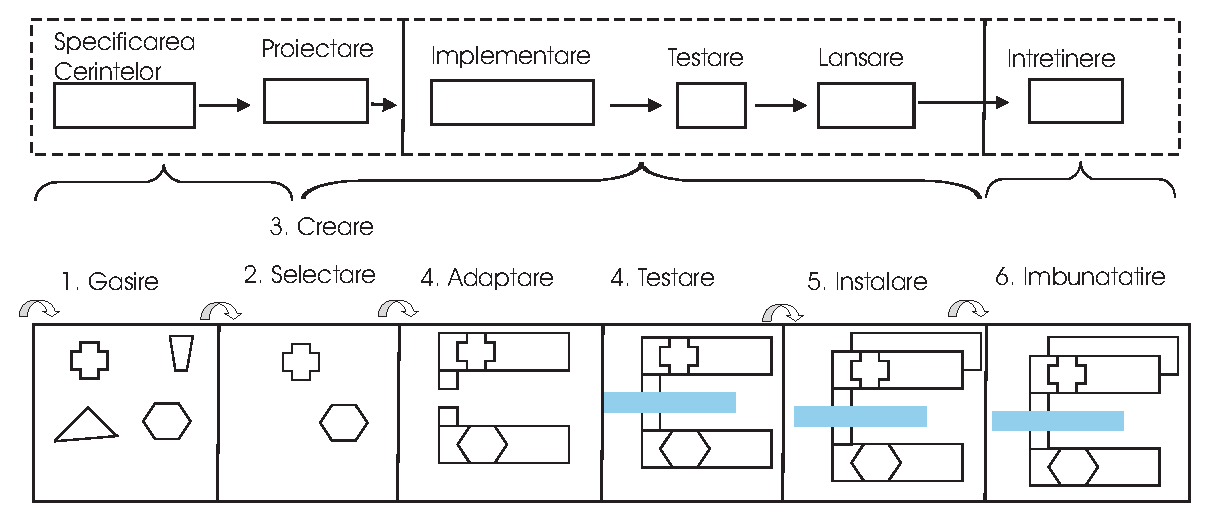
\includegraphics[scale=0.65]{Fig/fig_3_1.eps}
	\caption{Ciclul de dezvoltare al sistemelor bazate pe componente adaptat modelului cascad�}
	\label{Cap3Figura3-1}
\end{figure}


Referirea la Tabelul \ref{Cap3Tabel01}. 

\begin{table}[htbp]
\begin{center}
\begin{tabular}
{||p{100pt}||p{60pt}|p{60pt}||}
\hline
 Nume algoritm& 
 Toate solu�iile &
 Solu�ia optim�\\
\hline 
\hline Nume 1 & $20$ & $5$  \\
\hline Nume 2 & $20$ & $2$  \\
\hline
\end{tabular}
\end{center}
\caption{Solu�ii ob�inute }
\label{Cap3Tabel01}
\end{table}



\section{Prima sec�iune}

\subsection{Subsec�iunea unu}


Exemplu de prezentare algoritm.

\begin{algorithm}[htbp]
\begin{small}
\begin{algorithmic}  
\State \textbf{Input:}
\State {\ $\bullet$ the number $n$ ;}
\State {\ $\bullet$ the list $paramList$ of additional parameters that will be described in the proposed approaches.}
\State \textbf{Output:}
\State {\ $\bullet$ the solution.}
\State{}
\State {\textbf{Subalgorithm} \emph{IterativeBacktracking(n,[$paramListBack$])} is:}
\State \textbf{Begin}   
    \State {Let k := 1; possible[1] := \textit{init(1)};}   \Comment{initialise the search for the index k (=1)}
    \While {($k > 0$)}
    	\State {Let found := \textit{false}; v := possible[k];}
    	\While {( \textit{next(k,v,new)} \textbf{and} (not found))}
    			\State {Let v := new;}
    			\If {(\textit{conditionToContinue(k, possible,v,[$paramListCtC$])})}
    					\State { found := \textit{true};}
    			\EndIf    	
    	\EndWhile    
    	\If {(found)}
    			\State {Let possible[k] := v;}        \Comment{possible[1..k] is a solution candidate}
    			\If {(\textit{solution(n,k,possible,[$paramListSol$])})}          \Comment{found a solution}
    					\State {Print possible[1..k];}
    			\Else
    					\State { Let k := k+1;}     \Comment{step forward on level k+1}
    					\State {possible[k] := init(k);}
    			\EndIf    	
    	\Else
    			\State {k := k-1;}                 \Comment{step backward (backtrack to level k-1)}
    	\EndIf
    \EndWhile   
\State \textbf{End.}
\end{algorithmic}
\end{small}
\caption{The \textit{IterativeBacktracking} subalgorithm }
\label{AlgBackGeneral}
\end{algorithm}

\subsection{Subsec�iunea a doua}

\section{A doua sec�iune}


\chapter{Proposed approach}
\label{CapFT}

\section{Theoretical part}

\subsection{Architecture}

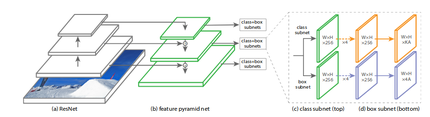
\includegraphics{Fig/arch1.png}

The model our work is based on is RetinaNet.
RetinaNet is a one stage detector having a convolutional neural network as a feature extractor for the 2 task-subnetworks it has. 
The first CNN's backbone is based on a Feature Pyramid Network build on a forward Residual Network. The FPN generates rich multi-scale feature 
maps. In [7] it is emphasised that we can also extract relevant features and make predictions based on feature maps that are on layers 
inside the network.
The pyramid usually has 7 levels.
The 2 task-subnetowrks are:
\begin{itemize}
  \item The classification subnetwork is a FCN that appears on each level of the pyramid and tries to classify each anchor box and outputing a K-vetor of probabilities for each class(meaning we have K classes).
  \item The box regression subnetwork has the same architecture (but different parameters) like the classification subnetwork only outputing a 4-vector representing the targets of the bounding box.
\end{itemize}

\subsection{The loss}

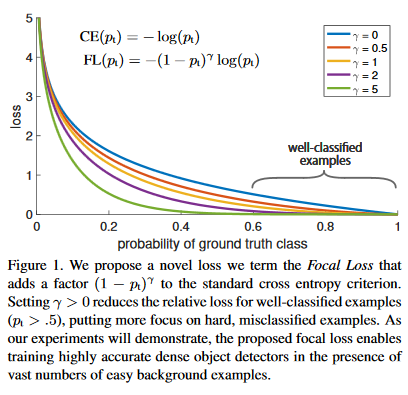
\includegraphics{Fig/focalloss.PNG}

Instead of the cross-entropy loss function we used a more novel loss function called the focal loss. The reason behind using focal loss is that (instead of using Online Hard Example Mining) the loss emphasies learning from hard examples.
The focal loss function stands at the end of the classification FCN and applied to all 100k anchor boxes sampled from a single image.

\section{Application development}


\chapter{Application}
\label{CapFT}

\section{Methodology}
I am Lord Voldemort
Absolventul va prezenta detaliat (pe baza document?rii bibliografice problematica tratat?:
soiangioionoinegoioinoin oinegwonai
\begin{itemize}
	\item ?ncadrarea temei ?ntr-una mai general?;
	\item trecerea ?n revist? a abord?rilor existente ale problemei cu marcarea avantajelor ?i dezavantajelor;
	\item descompunerea ?n subprobleme specifice ?i prezentarea modului de rezolvare.
\end{itemize}

\section{Dataset}

\section{Results}

\section{Discussion}

SCRIU AICIIII
	Partea fundament?rii teoretice poate fi consituit? din mai multe capitole, ca de exemplu ``Stadiul actual din domeniu/State of art/Literature Review'' ?i ``Modele teoretice ?i metode folosite/Research Method'' ?i ``Problem Statement''.





\chapter{Concluzii finale}
\label{CapCF}

Absolventul va realiza o autoevaluare a rezultatelor prezentate (punctarea aspectelor originale, a avantajelor �i limitelor solutiilor oferite) �i a eventualelor aspecte r�mase nerezolvate,

�n general se prezint� �n urm�toarele subsec�iuni: Concluzii, Sumarul contribu�iilor, Direc�ii viitoare de cercetare.

\section{Concluzii}

\section{Contribu�ii}

\section{Direc�ii viitoare de cercetare}



%ca sa apara bibliografia in contents
\clearpage
\addcontentsline{toc}{chapter}{Bibliografy}

\label{CapFT}

\begin{thebibliography}{9}
\bibitem{Goodfellow} 
Ian Goodfellow, et al.. 
\textit{Deep Learning}. 
MIT Press, Massachusetts, 2016.
 
\bibitem{Lungociu} 
Lungociu Corneliu
\textit{Real Time Sign Language Recognition Using Artificial Neural Networks}.
in Studia Univ. Babes-Bolyai, Informatica, Volume LVI, Number 4, 2011. 

\bibitem{Paranjape} 
Paranjape Ketki Vijay
\textit{Recent Developments in Sign Language Recognition: A Review}.
in International Journal on Advanced Computer Engineering and Communication Technology (IJACECT), Volume-1, Issue-2, 2012. 

\bibitem{Starner} 
T.Starner and A. Pentland
\textit{Real-Time American Sign Language Recognition from Video Using Hidden Markov Models}.
Computational Imaging and Vision, 9(1); 227-243, 1997.

\bibitem{Mekala} 
Mekala et al.
\textit{Real-Time Sign Language Recognition based on Neural Network Architecture}.
System Theory (SSST), 2011 IEEE 43rd Southeastern Symposium 14-16 March 2011. 

\bibitem{Brandon Garcia} 
Mekala et al.
\textit{Real-time American Sign Language Recognition with Convolutional Neural
Networks}.
Stanford Journal 2014
. 

\bibitem{Detectron}
Ross Girshick and Ilija Radosavovic and Georgia Gkioxari and Piotr Dollar and Kaiming He.
\textit{Detectron}
\\\texttt{https://github.com/facebookresearch/detectron}
\end{thebibliography}


\end{document}